\chapter{数据库系统简介}

\begin{introduction}[期末考试提纲]
    \item 数据独立性
    \item 文件系统在数据管理方面的不足
    \item 数据库系统在数据管理方面的特性
    \item 数据模型的概念、种类、特性比较
    \item 数据库模式:三级模式、两级映像

    \item 数据库是如何保证数据独立性的
    \item DBMS各项功能、DBA职责
\end{introduction}

\section{数据独立性}

\begin{definition}[数据结构]
按照逻辑关系组织起来的一批数据, 按一定的存储
方法把它存储在计算机中,
并在这些数据上定义了一个运算的集合.

\begin{enumerate}
    \item 逻辑结构: 数据之间存在的逻辑关系. e.g., 表、树、图.
    \item 物理结构: 数据在计算机内的存储方式. e.g., 顺序方式、链接方式.
\end{enumerate}
\end{definition}

\begin{definition}[数据独立性]
当数据结构发生变化时, 通过系统提供的
映象(转换)功能, 使应用程序不必改变.

\begin{enumerate}
    \item 数据的物理独立性: 当数据存储结构发生变化时, 使应用程序不必改变.
    \item 数据的逻辑独立性: 当数据逻辑结构发生变化时, 使应用程序不必改变.
\end{enumerate}
\end{definition}


数据定义: 逻辑结构、物理结构.

数据操作: 查询+更新.

数据约束: 对客观事物的合理反映, 数据一致性.

\section{数据管理发展阶段}

人工管理 $\to$ 文件系统 $\to$ 数据库系统 $\to$ 大数据时代

文件系统管理的不足:
\begin{enumerate}
    \item 数据定义独立性弱:
    \begin{enumerate}
        \item 数据与程序紧密结合;
        \item 数据的语义信息只能由程序来解释;
        \item 数据分散管理;
        \item 数据共享困难;
    \end{enumerate}
    \item 数据完整性难于维护(多副本);
    \item 数据查询困难(文件系统眼中的数据只是\textcolor{red}{字符流})
\end{enumerate}

数据库系统眼中的数据: \textcolor{red}{结构化数据}.

数据库系统保证\textcolor{red}{数据独立性}的举措:
\begin{enumerate}
    \item 把数据库定义和描述从应用程序中分离出去;
    \item 数据描述是分级的(全局逻辑、局部逻辑、存储);
    \item 数据存取由系统管理, 用户不必考虑存取路径等细节, 从而简化了应用程序(SQL).
\end{enumerate}

数据库具有统一的\textcolor{red}{数据控制}能力:
\begin{enumerate}
    \item 完整性控制
    \item 安全性控制
    \item 并发控制
    \item 恢复控制
\end{enumerate}

数据库系统的特点:
\begin{enumerate}
    \item 面向全组织, 有结构的数据, 记录之间无联系, 结构化数据
    \item 冗余度小, 集中管理, 易扩充性
    \item 高数据独立性
    \item 统一的数据控制功能: 安全性控制(security), 并发控制(concurrency), 完整性控制(integrity), 恢复控制(recovery)
\end{enumerate}


\section{数据模型}

\begin{definition}[数据模型]
    是数据库系统中用于提供信息表示和操作手段的形式构架.
\end{definition}

\begin{figure}[H]
    \centering
    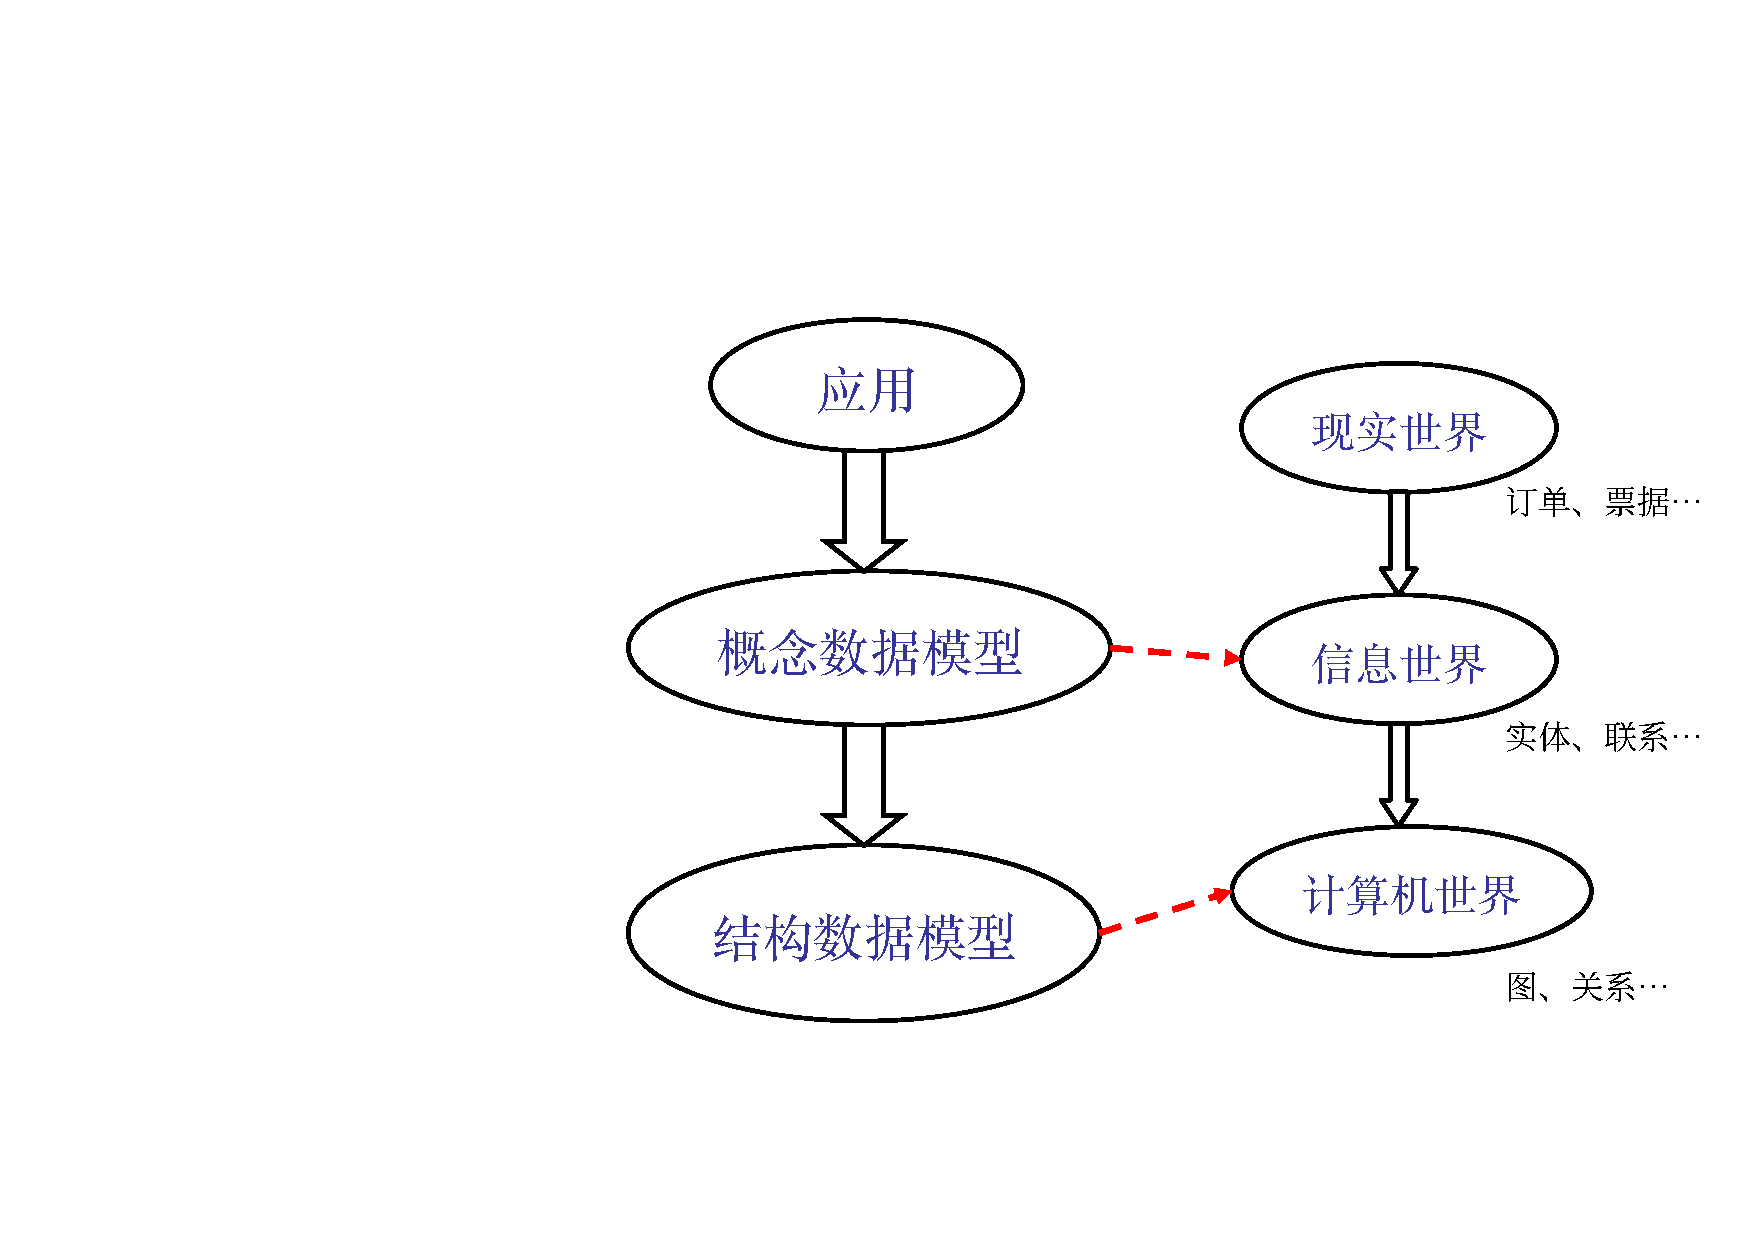
\includegraphics[width=.35\textwidth]{figure/数据模型.pdf}
    \caption{数据模型}
\end{figure}

概念模型: 强调语义表达能力, 给人看
\begin{enumerate}
    \item E-R(实体-联系模型, entity-relationship model).
    \item 基于对象的数据模型(object-based data model)
\end{enumerate}

结构数据模型的概念、种类、特性比较(强调数据结构, 计算机实现, 形式化定义, 给程序看.):
\begin{enumerate}
    \item 层次模型: 使用树状结构表示数据之间的关系, 每个记录只有一个父记录.
    \item 网络模型: 扩展了层次模型, 允许一个记录有多个父记录.
    \item 关系模型: 基于关系理论, 使用表格形式组织数据, 是目前最常用的数据模型.
    \item 面向对象模型: 将数据及其处理方法封装在一起, 支持复杂数据类型.
\end{enumerate}

\begin{figure}[H]
    \centering
    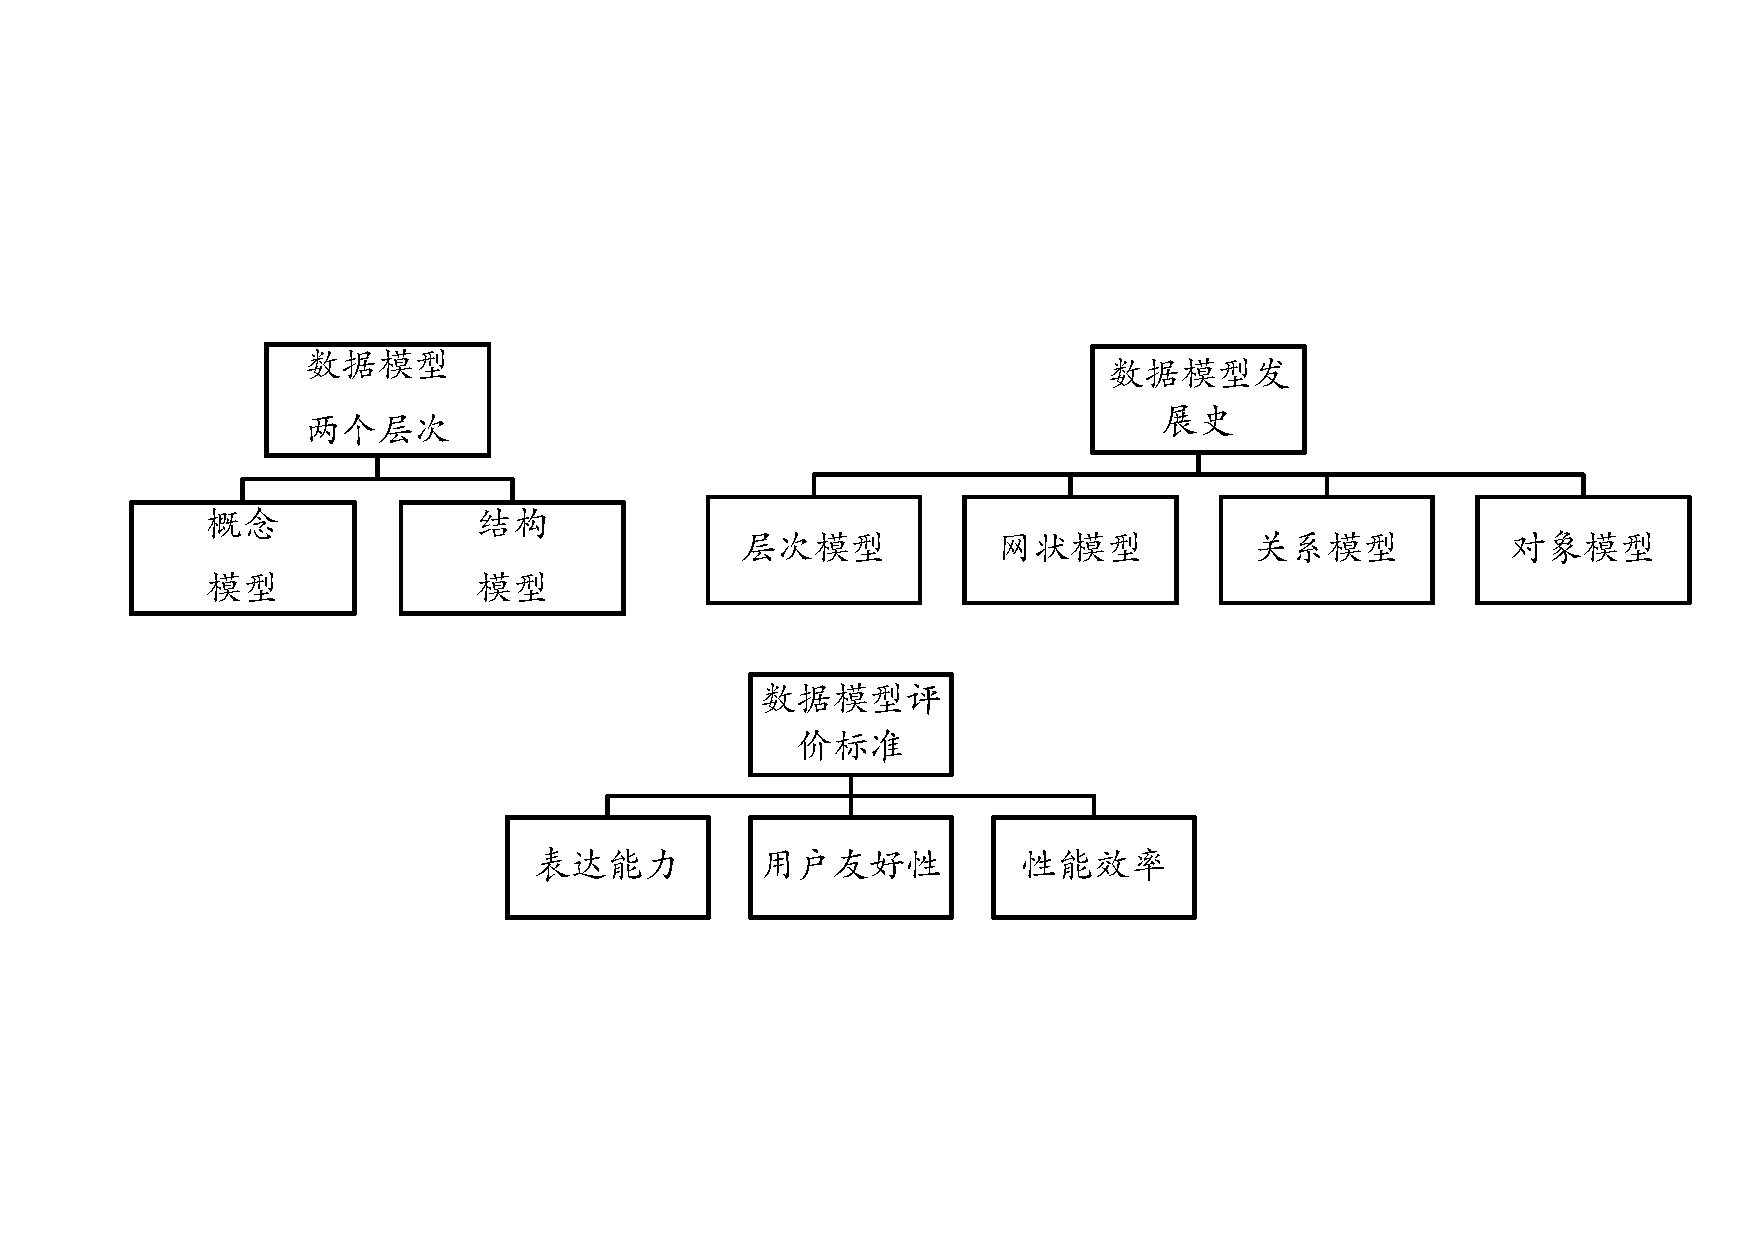
\includegraphics[width=.7\textwidth]{figure/db-5.pdf}
    \caption{数据模式总结}
\end{figure}

\begin{definition}[元数据(metadata)]
元数据是\textcolor{red}{描述数据的数据}.
\end{definition}

所谓\textcolor{red}{数据库模式}, 实际上是一种类型, 而它的值就是数据库当前的一个快照.

数据库系统的架构通常遵循\textcolor{red}{三级模式}和\textcolor{red}{两级映像}的原则.
\begin{enumerate}
    \item 外模式(视图层): 用户看到并与之交互的数据视图.
    \item 模式(逻辑层): 描述数据库中数据的整体逻辑结构.
    \item 内模式(物理层): 定义数据的实际存储方式和访问路径.
    \item 两级映像指的是\textit{外模式/模式映像}和\textit{模式/内模式映像}, 用于保证数据独立性
    \begin{itemize}
        \item 外模式/模式映像: 定义某个外模式和模式之间的对应关系
        \item 模式/内模式映像: 定义数据逻辑结构与存储结构之间的对应关系
    \end{itemize}
\end{enumerate}

\textit{我的理解: 所谓外模式映像就是定义这样一个映射$f$把当前的view映射到某个表上, 内模式映像则是一个映射$g$将某个table映射到存储结构上.}

\begin{figure}[H]
    \centering
    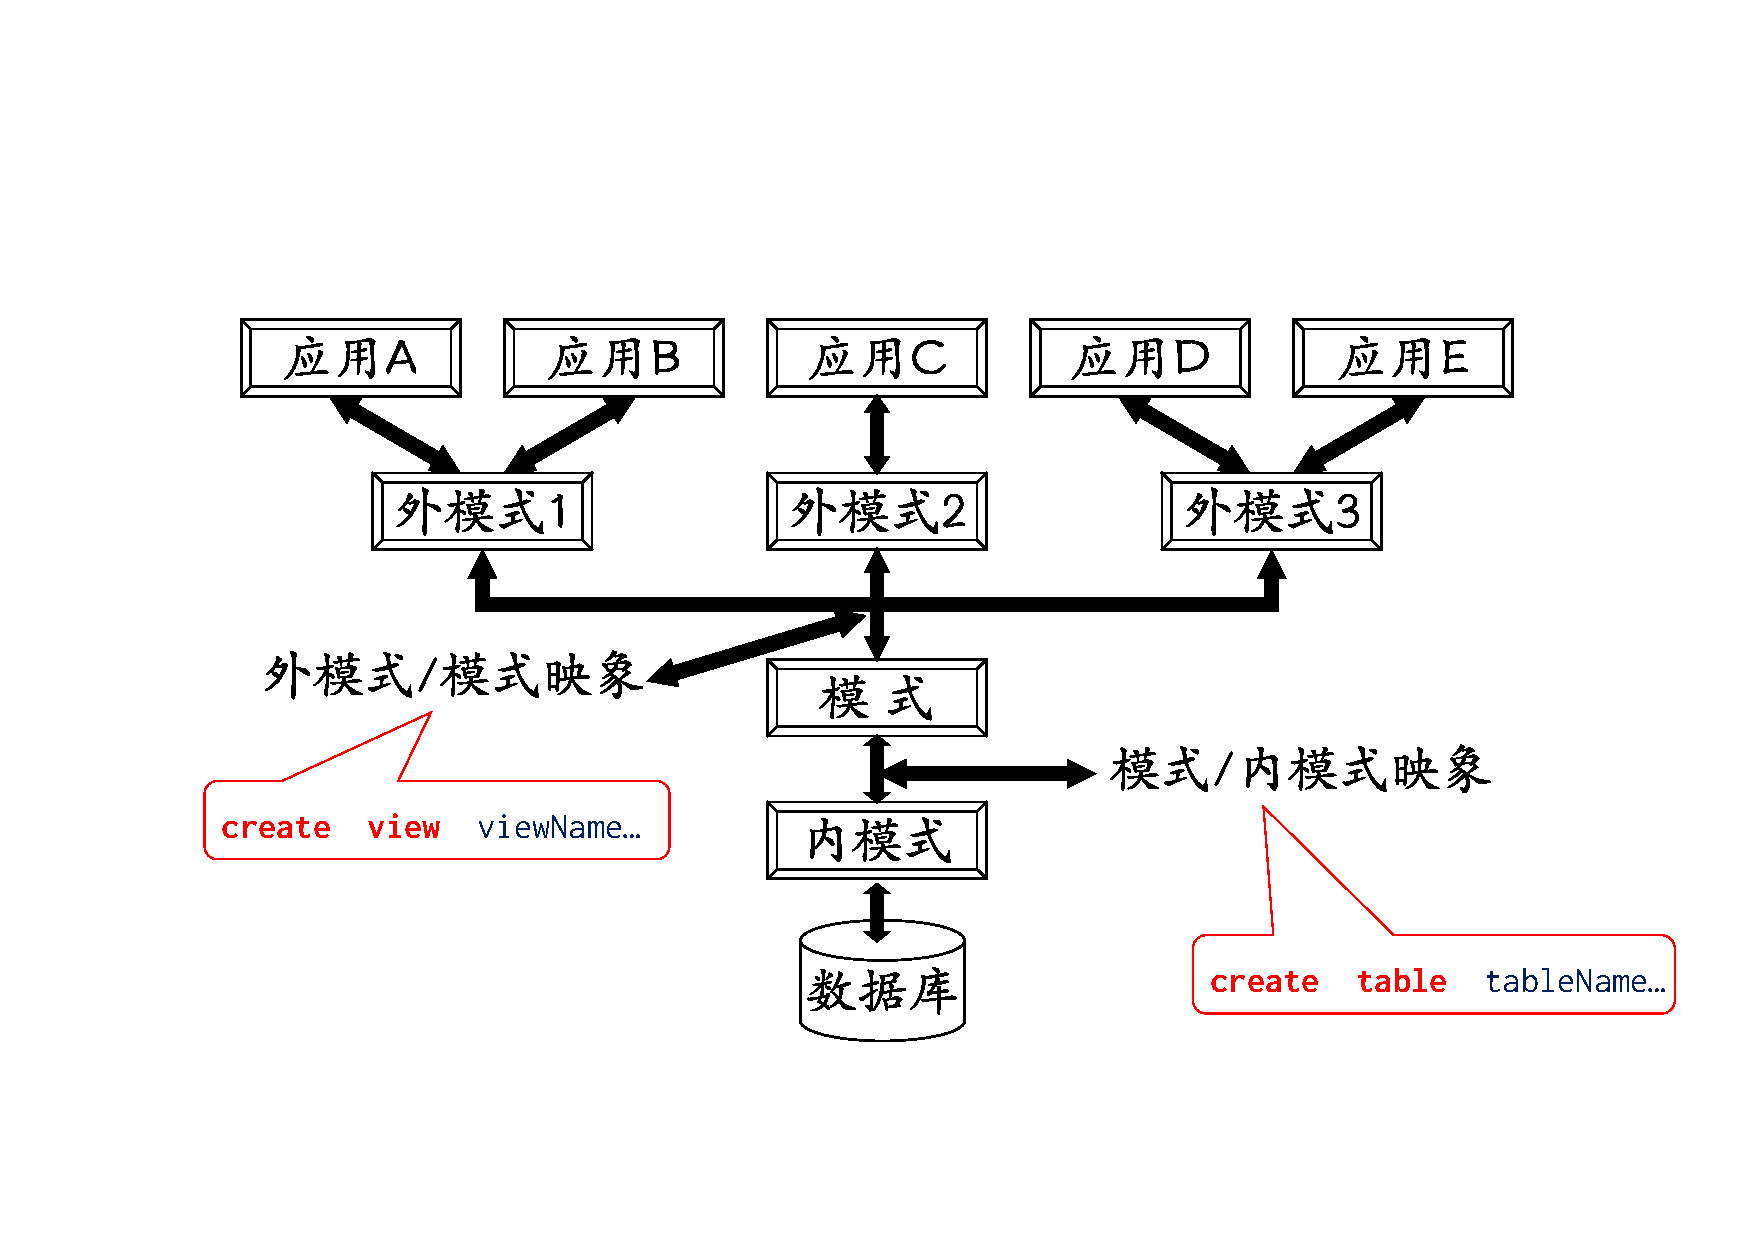
\includegraphics[width=.6\textwidth]{figure/db-6.pdf}
    \caption{数据库的三种模式}
\end{figure}

\begin{remark}
    数据库的逻辑独立性来自于: 外模式/模式映像. 数据库的物理独立性来自于: 模式/内模式映像.
\end{remark}

\begin{figure}[H]
    \centering
    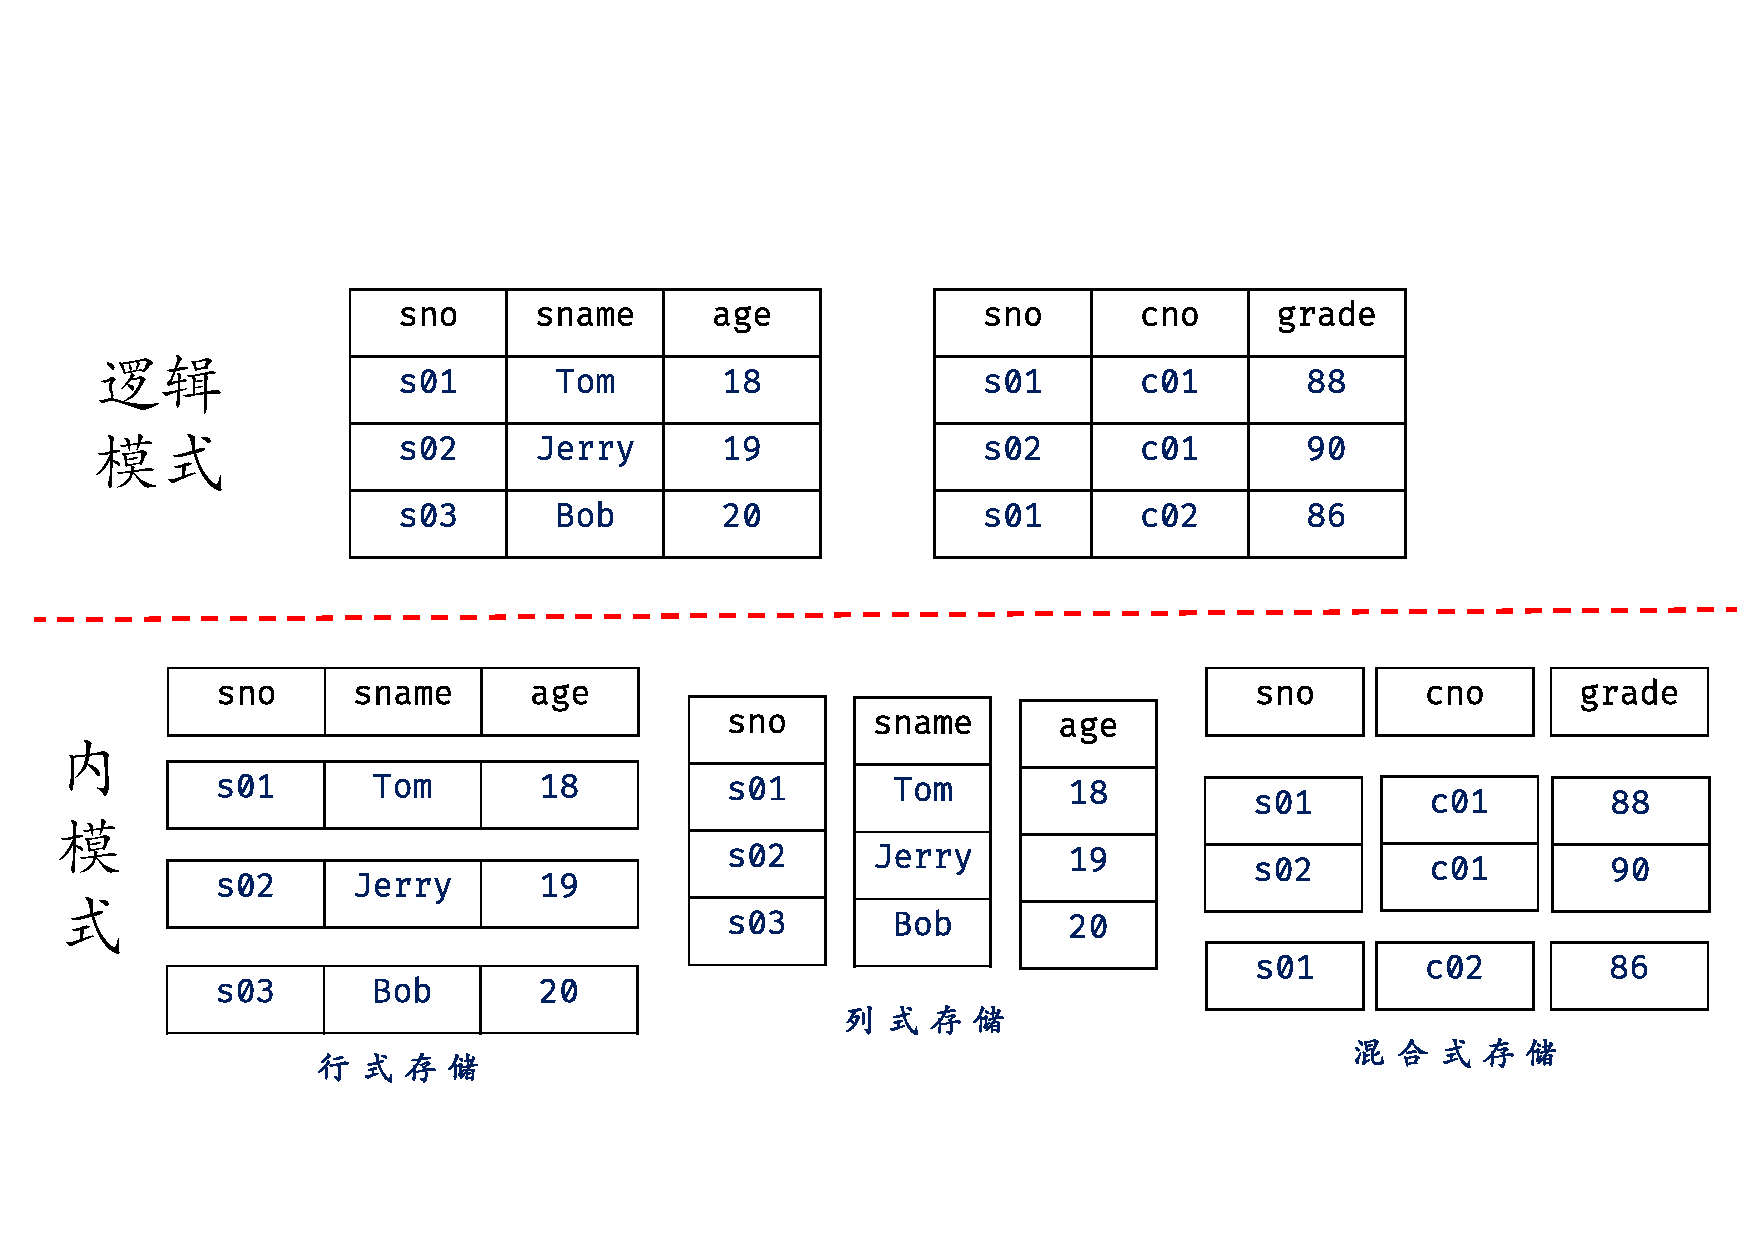
\includegraphics[width=.8\textwidth]{figure/内模式.pdf}
    \caption{数据库内模式的例子}
\end{figure}

\section{数据库系统的构成}

\begin{definition}[数据库]
    数据的集合. 由DBMS统一管理, 多用户共享.
\end{definition}

\begin{definition}[数据库管理系统DBMS]
    系统软件, 对数据库进行统一管理和控制.
\end{definition}

\begin{definition}[数据库系统]
    带有数据库的整个计算机系统, 包括硬件、软件、数据、人员.
\end{definition}

DBMS(数据库管理系统)的功能包括但不限于:
\begin{itemize}
    \item 数据定义: 创建、修改和删除数据库中的对象.
    \item 数据操作: 插入、更新、删除和查询数据库中的数据.
    \item 数据库事务管理: 确保数据库操作的原子性、一致性、隔离性和持久性(ACID属性).
    \item 数据库备份与恢复: 提供机制以防止数据丢失, 并在必要时恢复数据.
\end{itemize}

DBA(数据库管理员)的职责:
\begin{itemize}
    \item 建库方面: 确定模式、外模式、存储结构、存取策略; 负责数据的整理和装入.
    \item 用库方面: 
    \begin{itemize}
        \item 定义完整性约束条件
        \item 规定数据的保密级别、用户权限
        \item 监督和控制数据库的运行情况
        \item 制定后援和恢复策略, 负责故障恢复
    \end{itemize}
    \item 改进方面:
    \begin{itemize}
        \item 监督分析系统的性能(空间利用率, 处理效率)
        \item 数据库重组织, 物理上重组织, 以提高性能
        \item 数据库重构造, 设计上较大改动, 模式和内模式修改
    \end{itemize}
\end{itemize}
